\documentclass{scu-thesis}

%%%%%%%%%%%%%%%%%%%%%%%%%%%%%%%%%%%%%%%%%%%%%%%%%%%%%%%%%%%%%%%%%%%%%%%
%% User settings %%%%%%%%%%%%%%%%%%%%%%%%%%%%%%%%%%%%%%%%%%%%%%%%%%%%%%
%%%%%%%%%%%%%%%%%%%%%%%%%%%%%%%%%%%%%%%%%%%%%%%%%%%%%%%%%%%%%%%%%%%%%%%

% English digits in equations and tikz
% \DefaultMathsDigits

% Two columns footnotes
\twocolumnfootnotes

% Hide borders of hyperlinks
% \hypersetup {hidelinks}

% Using tikz positioning
\usetikzlibrary{positioning}

% Nastaliq font (you must install IranNastaliq font before using this command)
% \defpersianfont\nastaliq{IranNastaliq}

%%%%%%%%%%%%%%%%%%%%%%%%%%%%%%%%%%%%%%%%%%%%%%%%%%%%%%%%%%%%%%%%%%%%%%%
%% Read user input files %%%%%%%%%%%%%%%%%%%%%%%%%%%%%%%%%%%%%%%%%%%%%%
%%%%%%%%%%%%%%%%%%%%%%%%%%%%%%%%%%%%%%%%%%%%%%%%%%%%%%%%%%%%%%%%%%%%%%%

% Input the cover information
%!TEX root = ../thesis.tex

% Package URL: https://github.com/hanifbirgani/scu-thesis-latex

% در این فایل اطلاعات لازم جهت صفحه‌چینی پایان‌نامه وارد شود

%%%%%%%%%%%%%%%%%%%%%%%%%%%%%%%%%%%%%%%%%%%%%%%%%%%%%%%%%%%%%%%%%%%%%%%
% مقادیر فارسی %%%%%%%%%%%%%%%%%%%%%%%%%%%%%%%%%%%%%%%%%%%%%%%%%%%%%%%%
%%%%%%%%%%%%%%%%%%%%%%%%%%%%%%%%%%%%%%%%%%%%%%%%%%%%%%%%%%%%%%%%%%%%%%%
% عنوان دانشجو: آقای / خانم
\authorTitle{آقای}
% نام کوچک دانشجو
\authorFirstname{حنیف}
% نام خانوادگی دانشجو
\authorLastname{تقی‌پور بیرگانی}
% شماره دانشجویی
\studentID{92939495}
% عنوان پایان‌نامه
\reportTitle{کلاس لاتک پایان‌نامه دانشگاه شهید چمران اهواز}
% نام دانشکده
\faculty{مهندسی}
% لینک دانشکده - اختیاری
\facultyLink{}
% گروه تحصیلی
\departement{کامپیوتر}
% لینک گروه تحصیلی - اختیاری
\departementLink{}
% مقطع تحصیلی
\degreeType{کارشناسی ارشد}
% رشته
\major{مهندسی کامپیوتر}
% گرایش
\field{هوش مصنوعی و رباتیک}
% نوع سند: پایان‌نامه / رساله
\reportType{پایان‌نامه}
% شماره پایان‌نامه - پس از گرفتن وقت دفاع، می‌توانید این شماره را از آموزش دریافت کنید
\thesisID{123456}
% لینک سایت شخصی دانشجو - اختیاری
\authorLink{https://HanifBirgani.com}
% درجه ارزیابی پایان‌نامه -  نتیجه ارزیابی پس از نمره دفاع مشخص می‌شود
\evaluationRate{عالی}
% تاریخ دفاع - ماه (حروف) و سال (عدد چهار رقمی) فارسی
\reportDate{شهریور ۱۳۹۵}
% تاریخ دفاع عددی - روز/ماه/سال
\graduationDate{1395/6/31}
% کلیدواژه‌ها
\keywords{واژه اول، واژه دوم، واژه سوم و...}
% نام کامل استاد راهنما
\supervisor{نام دکتر استاد راهنما}
% درجه استاد راهنما
\supervisorGrade{استادیار}
% نام کامل استاد راهنمای دوم - اختیاری
\supervisorSecond{}
% درجه استاد راهنمای دوم - اختیاری
\supervisorSecondGrade{}
% نام کامل استاد مشاور
\advisor{نام دکتر استاد مشاور}
% درجه استاد مشاور
\advisorGrade{استادیار}
% نام کامل استاد مشاور دوم - اختیاری
\advisorSecond{}
% درجه استاد مشاور دوم - اختیاری
\advisorSecondGrade{}
% نام کامل داور اول
\examinerFirst{نام دکتر داور اول}
% درجه داور اول
\examinerFirstGrade{استادیار}
% نام کامل داور دوم
\examinerSecond{نام دکتر داور دوم}
% درجه داور دوم
\examinerSecondGrade{استادیار}
% نام کامل داور سوم - اختیاری
\examinerThird{}
% درجه داور سوم - اختیاری
\examinerThirdGrade{}
% نام کامل نماینده دانشکده
\graduateRepresenter{نام دکتر نماینده دانشکده}
% درجه نماینده دانشکده
\graduateRepresenterGrade{استاد}
% نام کامل مدیر گروه
\departmentHead{نام دکتر مدیر گروه}
% درجه مدیر گروه
\departmentHeadGrade{استادیار}
% نام کامل مدیر تحصیلات تکمیلی دانشگاه
\graduateDirector{نام دکتر مدیر تحصیلات تکمیلی}
% درجه مدیر تحصیلات تکمیلی دانشگاه
\graduateDirectorGrade{استاد}
% نام کامل معاون آموزشی دانشکده
\graduateAssistant{نام دکتر معاون آموزشی دانشکده}
% درجه معاون آموزشی دانشکده
\graduateAssistantGrade{دانشیار}

%%%%%%%%%%%%%%%%%%%%%%%%%%%%%%%%%%%%%%%%%%%%%%%%%%%%%%%%%%%%%%%%%%%%%%%
% English Values %%%%%%%%%%%%%%%%%%%%%%%%%%%%%%%%%%%%%%%%%%%%%%%%%%%%%%
%%%%%%%%%%%%%%%%%%%%%%%%%%%%%%%%%%%%%%%%%%%%%%%%%%%%%%%%%%%%%%%%%%%%%%%

% Student firstname
\authorFirstnameEnglish{Hanif}
% Student lastname
\authorLastnameEnglish{Taghipour Birgani}
% Thesis title
\reportTitleEnglish{\LaTeX{} Class for Shahid Chamran University of Ahvaz}
% Faculty name
\facultyEnglish{Engineering}
% Department name
\departementEnglish{Computer Engineering}
% Degree type
\degreeTypeEnglish{Master of Artificial Intelligence and Robotics}
% Major
\majorEnglish{Computer Engineering}
% Document type
\reportTypeEnglish{Thesis}
% Field of study
\fieldEnglish{Artificial Intelligence and Robotics}
% Supervisor fullname
\supervisorEnglish{Dr. Supervisor}
% Second Supervisor fullname - Optional
\supervisorSecondEnglish{}
% Advisor fullname
\advisorEnglish{Dr. Advisor}
% Second Advisor fullname - Optional
\advisorSecondEnglish{}
% Report date in Month (alphabetic) Year (numerical) format
\reportDateEnglish{September 2019}
% Report date in numerical format YYYY/MM/DD
\graduationDateEnglish{2019/9/10}
% Keywords
\keywordsEnglish{First keyword, Second keyword, Third keyword, ...}

% Glossary inputs
%!TEX root = ../thesis.tex

%%%%%%%%%%%%%%%%%%%%%%%%%%%%%%%%%%%%%%%%%%%%%%%%%%%%%%%%%%%%%%%%%%%%%%%
%% Define Words %%%%%%%%%%%%%%%%%%%%%%%%%%%%%%%%%%%%%%%%%%%%%%%%%%%%%%%
%%%%%%%%%%%%%%%%%%%%%%%%%%%%%%%%%%%%%%%%%%%%%%%%%%%%%%%%%%%%%%%%%%%%%%%
% \newword{word_reference}{Word}{ترجمه واژه در حالت تکی}{ترجمه واه در حالت جمع}

\newword{optimizer}{Optimizer}{بهینه‌ساز}{بهینه‌سازها}
\newword{kernel}{Kernel}{هسته}{هسته‌ها}



%%%%%%%%%%%%%%%%%%%%%%%%%%%%%%%%%%%%%%%%%%%%%%%%%%%%%%%%%%%%%%%%%%%%%%%
%% Define Abbreviations %%%%%%%%%%%%%%%%%%%%%%%%%%%%%%%%%%%%%%%%%%%%%%%
%%%%%%%%%%%%%%%%%%%%%%%%%%%%%%%%%%%%%%%%%%%%%%%%%%%%%%%%%%%%%%%%%%%%%%%

\newacronym{cnn}{CNN}{Convolution Neural Network}
\newacronym{mse}{MSE}{Mean Square Error}

% Abstracts
%!TEX root = ../thesis.tex

\abstractPersian{% DO NOT TOUCH THIS LINE
    لورم ایپسوم متن ساختگی با تولید سادگی نامفهوم از صنعت چاپ و با استفاده از طراحان گرافیک است. چاپگرها و متون بلکه روزنامه و مجله در ستون و سطرآنچنان که لازم است و برای شرایط فعلی تکنولوژی مورد نیاز و کاربردهای متنوع با هدف بهبود ابزارهای کاربردی می باشد. کتابهای زیادی در شصت و سه درصد گذشته، حال و آینده شناخت فراوان جامعه و متخصصان را می طلبد تا با نرم افزارها شناخت بیشتری را برای طراحان رایانه ای علی الخصوص طراحان خلاقی و فرهنگ پیشرو در زبان فارسی ایجاد کرد. در این صورت می توان امید داشت که تمام و دشواری موجود در ارائه راهکارها و شرایط سخت تایپ به پایان رسد وزمان مورد نیاز شامل حروفچینی دستاوردهای اصلی و جوابگوی سوالات پیوسته اهل دنیای موجود طراحی اساسا مورد استفاده قرار گیرد.

    لورم ایپسوم متن ساختگی با تولید سادگی نامفهوم از صنعت چاپ و با استفاده از طراحان گرافیک است. چاپگرها و متون بلکه روزنامه و مجله در ستون و سطرآنچنان که لازم است و برای شرایط فعلی تکنولوژی مورد نیاز و کاربردهای متنوع با هدف بهبود ابزارهای کاربردی می باشد. کتابهای زیادی در شصت و سه درصد گذشته، حال و آینده شناخت فراوان جامعه و متخصصان را می طلبد تا با نرم افزارها شناخت بیشتری را برای طراحان رایانه ای علی الخصوص طراحان خلاقی و فرهنگ پیشرو در زبان فارسی ایجاد کرد. در این صورت می توان امید داشت که تمام و دشواری موجود در ارائه راهکارها و شرایط سخت تایپ به پایان رسد وزمان مورد نیاز شامل حروفچینی دستاوردهای اصلی و جوابگوی سوالات پیوسته اهل دنیای موجود طراحی اساسا مورد استفاده قرار گیرد.
    

}% DO NOT TOUCH THIS LINE
%!TEX root = ../thesis.tex

\abstractEnglish{% DO NOT TOUCH THIS LINE
    Lorem ipsum dolor sit amet, consectetur adipiscing elit. Maecenas odio neque, blandit a ante sit amet, viverra tincidunt leo. Nulla sed turpis pharetra, viverra erat vitae, lacinia mi. Donec iaculis diam at turpis consectetur, ac eleifend diam vehicula. Nam fringilla fringilla dictum. Aenean et dolor bibendum nisi feugiat gravida. Fusce volutpat vehicula magna, quis aliquet ipsum interdum ut. Suspendisse vitae urna leo. Etiam vulputate ut leo et ornare. Etiam laoreet tortor tellus, quis pellentesque risus facilisis nec. Vivamus venenatis eu ex quis pretium.

    Suspendisse in leo non elit hendrerit ornare. Vestibulum ultrices sollicitudin massa et accumsan. Curabitur luctus libero neque, sed tempus odio vulputate eget. Etiam augue nisi, feugiat sed nulla vitae, faucibus blandit quam. Mauris nibh lectus, tempor ac eleifend quis, consequat vel libero. Aenean et massa sed sapien ullamcorper dictum a pretium eros. Vestibulum malesuada magna ac nunc sagittis, ac finibus ipsum lacinia. Praesent ultricies lacus sit amet felis facilisis egestas. Mauris interdum tempus gravida. Vivamus at diam erat.
    
    
}% DO NOT TOUCH THIS LINE


%%%%%%%%%%%%%%%%%%%%%%%%%%%%%%%%%%%%%%%%%%%%%%%%%%%%%%%%%%%%%%%%%%%%%%%
%% Generate the document %%%%%%%%%%%%%%%%%%%%%%%%%%%%%%%%%%%%%%%%%%%%%%
%% DO NOT EDIT without knowing what you are doing! %%%%%%%%%%%%%%%%%%%%
%%%%%%%%%%%%%%%%%%%%%%%%%%%%%%%%%%%%%%%%%%%%%%%%%%%%%%%%%%%%%%%%%%%%%%%

\begin {document}
	
	% Besmellah page
	% Put your besmellah file in images directory. Supported formats: jpg, png, pdf, eps
	% File name MUST be "besmellah" (all in lowercase)
	\printBesmellah
	
	% Persian Cover page
	\makeCoverPersian

	% Evaluation page
	\makeEvaluation
	
	% Originality page
	\makeOriginality

	% Dedication page
	%!TEX root = ../thesis.tex

\thispagestyle{empty}% DO NOT TOUCH THIS LINE

تقدیم به شما
	
	% Acknowledgements page
	%!TEX root = ../thesis.tex

\thispagestyle{empty}% DO NOT TOUCH THIS LINE

با سپاس از همه

	% Persian abstract page
	\makeAbstractPersian
	
	% Table of contents
    \makeTableOfContents
	
	% List of figures
    \makeListOfFigures

	% List of tables
    \makeListOfTables
	
	% Do NOT remove or comment the line below
    \startChapters% DON'T TOUCH
    
    % Chapters
	%!TEX root = ../../thesis.tex

\chapter{مقدمه} \label{chapter:introduction}

محتوای فصل اول به صورت نمونه در خطوط زیر قرار گرفته است.

شما در حال مشاهده نگارش $2.0.0$ از قالب لاتک پایان‌نامه دانشگاه چمران اهواز هستید. جهت دریافت جدیدترین نگارش به آدرس زیر مراجعه کنید:

\begin{center}
	\href{https://github.com/hanifbirgani/scu-thesis-latex}{https://github.com/hanifbirgani/scu-thesis-latex}
\end{center}



دانشگاه شهید چمران اهواز یک دانشگاه دولتی در کلان‌شهر اهواز، چهارمین دانشگاه بزرگ کشور و بزرگ‌ترین دانشگاه در جنوب ایران است. دانشگاه شهید چمران به دلیل امکانات گسترده و فضای آموزشی بسیار وسیع از معتبرترین دانشگاه‌های ایران می‌باشد. این دانشگاه با ۱۵ دانشکده و ۱ پردیس دانشگاهی، یکی از ۱۰ دانشگاه برتر جامع کشور محسوب می‌شود که در سال ۱۳۳۲ تأسیس شد. نام قدیم این دانشگاه جندی شاپور بوده‌است. مطابق ارزیابی‌های وزارت علوم، دانشگاه شهید چمران اهواز یکی از دانشگاه‌های «سطح یک» کشور به‌شمار می‌رود.
%==SECTION==%
\section{تاریخچه}\label{sec:history}

قدمت دانشگاه جندی‌شاپور، به سدهٔ چهارم یا پنجم میلادی بازمی‌گردد و در طی ۶ قرن، نام جندی‌شاپور مترادف با مرکزی علمی در رشته‌های مختلف بوده‌است و عصر تعالی و ترقی آن در زمان خسرو انوشیروان بوده‌است. مکان شهر دانشگاهی جندی‌شاپور در دوران ایران باستان به‌طور قطعی مشخص نیست، اما به گفته احمد اقتداری از منابع گوناگون برمی‌آید که در محدوده میان شهرهای شوشتر، شوش و دزفول قرار داشته‌است.\cite{eghtedari00diyar}

دانشگاهی با نام گندی‌شاپور در یکشنبه ۲ مهر ماه سال ۱۳۳۴ در اهواز گشایش یافت. پس از چندی این نام به جندی‌شاپور تغییر کرد. دانشگاه در نزدیکی رودخانهٔ کارون، در زمینی هموار و نزدیک باغ گیاهان گرمسیری بنا گردید. به دلیل طراحی چندین بنا و دانشکده توسط معمارانی نظیر کامران دیبا و آندره گدار، ساختمان این دانشگاه، از معماری منحصر به فردی برخوردار است.

مرجع \cite{Omidali82phdThesis} یک نمونه پروژه دکترا و مرجع \cite{Vahedi87} یک نمونه مقاله مجله فارسی است.
مرجع \cite{Amintoosi87afzayesh}  یک نمونه  مقاله کنفرانس فارسی و
مرجع \cite{Pedram80osool} یک نمونه کتاب فارسی با ذکر مترجمان و ویراستاران فارسی است. مرجع \cite{Khalighi07MscThesis} یک نمونه پروژه کارشناسی ارشد انگلیسی و
\cite{Khalighi87xepersian} هم یک نمونه متفرقه  می‌باشند.

مرجع \cite{Gonzalez02book} یک نمونه کتاب لاتین است که از آنجا که دارای فیلد \lr{authorfa} است، نام نویسندگان آن در استیلهای \lr{asa-fa}، \lr{plainnat-fa} و \lr{chicago-fa} به فارسی دیده می‌شود. مرجع \cite{Baker02limits} مقاله انگلیسی است که معادل فارسی نام نویسندگان آن ذکر نشده بوده است.



%==SUBSECTION==%
\subsection{معادله ریاضی}\label{sec:math-equation}
نمونه یک فرمول ریاضی در لاتک را در خطوط بعدی مشاهده خواهید کرد:

\begin{equation}
	\label{eq:a}
    J(\theta)=\frac{1}{2 m} \sum\left(h_{\theta}\left(x^{(i)}\right)-y^{(i)}\right)^{2}
\end{equation}

%==SUBSECTION==%
\subsection{تصویر نمونه}\label{sec:sample-image}
یک تصویر نمونه را در لاتک مشاهده می‌کنید.

\begin{figure}[H]
    \label{fig:main-gate}
    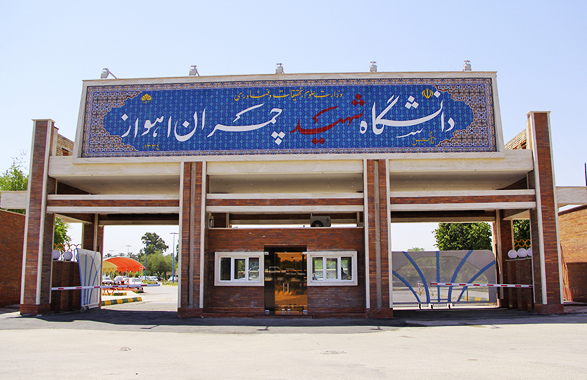
\includegraphics[width=0.5\textwidth]{chapter01/scu_main_gate}
    \caption{سردر غربی دانشگاه چمران}
\end{figure}

\subsection{تصویر چندتایی}\label{sec:multi-image}
\begin{figure}[H]
	\begin{subfigure}[t]{5cm}
		\centering
		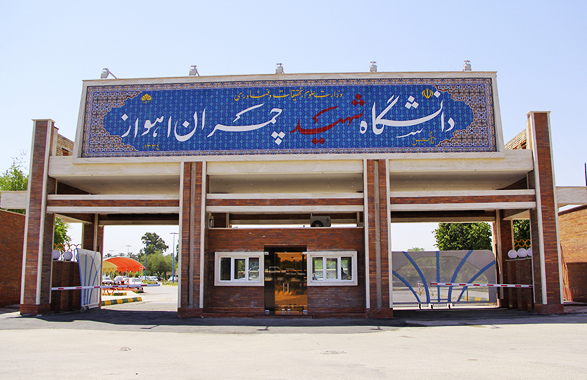
\includegraphics[width=5cm]{chapter01/scu_main_gate}
		\caption{ورودی شمالی}\label{fig:1a}		
	\end{subfigure}
	\quad
	\begin{subfigure}[t]{5cm}
		\centering
		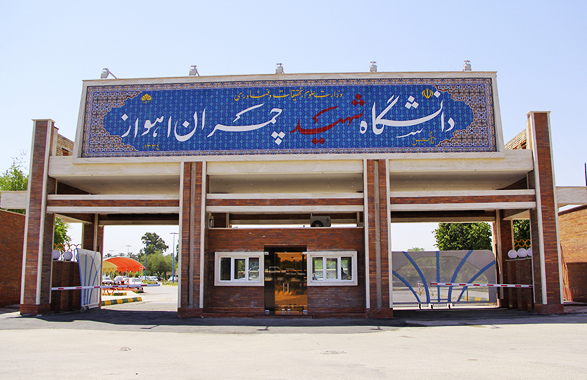
\includegraphics[width=5cm]{chapter01/scu_main_gate}
		\caption{ورودی جنوبی}\label{fig:1b}
	\end{subfigure}
	\caption{ورودی‌های دانشگاه چمران}\label{fig:1}
\end{figure}


\section{نمودار}

\begin{figure}[H]
	\begin{tikzpicture}
		\begin{loglogaxis}[
			xlabel=هزینه,
			ylabel=خطا]
		\addplot coordinates {
			(5,     8.31160034e-02)
			(17,    2.54685628e-02)
			(49,    7.40715288e-03)
			(129,   2.10192154e-03)
			(321,   5.87352989e-04)
			(769,   1.62269942e-04)
			(1793, 4.44248889e-05)
			(4097, 1.20714122e-05)
			(9217, 3.26101452e-06)
		};
		\addplot plot coordinates {
			(7,     8.47178381e-02)
			(31,    3.04409349e-02)
			(111,   1.02214539e-02)
			(351,   3.30346265e-03)
			(1023,  1.03886535e-03)
			(2815,  3.19646457e-04)
			(7423,  9.65789766e-05)
			(18943, 2.87339125e-05)
			(47103, 8.43749881e-06)
		};
		\legend{\rl{حالت ۱},\rl{حالت ۲}}
		\end{loglogaxis}
	\end{tikzpicture}
	\caption{مثال}
\end{figure}

\subsection{رسم انتگرال یک تابع}\label{sec:math-plot}
\begin{figure}[H]
    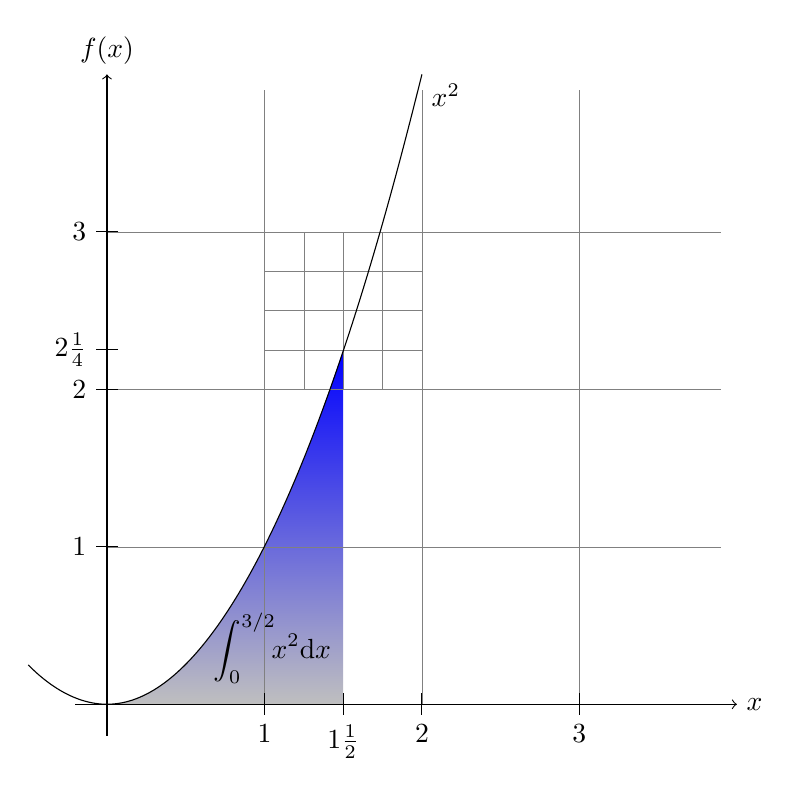
\begin{tikzpicture}[scale=2]
        \shade[top color=blue,bottom color=gray!50] 
            (0,0) parabola (1.5,2.25) |- (0,0);
        \draw (1.05cm,2pt) node[above] 
            {$\displaystyle\int_0^{3/2} \!\!x^2\mathrm{d}x$};

        \draw[style=help lines] (0,0) grid (3.9,3.9)
                [step=0.25cm]      (1,2) grid +(1,1);

        \draw[->] (-0.2,0) -- (4,0) node[right] {$x$};
        \draw[->] (0,-0.2) -- (0,4) node[above] {$f(x)$};

        \foreach \x/\xtext in {1/1, 1.5/1\frac{1}{2}, 2/2, 3/3}
            \draw[shift={(\x,0)}] (0pt,2pt) -- (0pt,-2pt) node[below] {$\xtext$};

        \foreach \y/\ytext in {1/1, 2/2, 2.25/2\frac{1}{4}, 3/3}
            \draw[shift={(0,\y)}] (2pt,0pt) -- (-2pt,0pt) node[left] {$\ytext$};

        \draw (-.5,.25) parabola bend (0,0) (2,4) node[below right] {$x^2$};
    \end{tikzpicture}
\end{figure}

\section{علائم و اختصارات}

مثلا \gls{optimizer}
مثلا \gls{kernel}
مثلا \gls{mse}
مثلا \gls{cnn}

	%!TEX root = ../../thesis.tex

\chapter{پیشینه پژوهش و مبانی نظری} \label{chapter:related-works}

محتوای فصل دوم
	%!TEX root = ../../thesis.tex

\chapter{روش پیشنهادی} \label{chapter:proposed-method}

محتوای فصل سوم
	%!TEX root = ../../thesis.tex

\chapter{پیاده‌سازی و ارزیابی نتایج} \label{chapter:evaluation}

محتوای فصل چهارم
    %!TEX root = ../../thesis.tex

\chapter{نتیجه‌گیری} \label{chapter:conclusion}

محتوای فصل پنجم
    
    % References
    \bibliographystyle{plain-fa}
    \makeBibliography

    % Glossary and Abbreviations
	% Uncomment two below lines to print Glossary and Abbreviations
    % \printglossary
    % \printabbreviation

	% Do NOT remove or comment the line below
    \closeChapters% DON'T TOUCH
    
	% English sections
	\begin{latin}

		% English abstract page
		\makeAbstractEnglish
		
		% English cover page
		\makeCoverEnglish

	\end{latin}

\end {document}